\documentclass[aspectratio=169]{beamer}
\usetheme{Madrid}
\usepackage[utf8]{inputenc}
\usepackage[T1]{fontenc}
\usepackage{lmodern}
\usepackage{booktabs}
\usepackage{array}
\usepackage{ragged2e}
\usepackage{hyperref}
\usepackage{setspace}

\usepackage{tabularx}
\newcolumntype{Y}{>{\raggedright\arraybackslash}X}

\usepackage{float}
\usepackage{array}
\usepackage{graphicx}
\usepackage[table]{xcolor}
\usepackage{svg}
\usepackage{tikz}
\usetikzlibrary{arrows.meta, positioning, fit, backgrounds}

\definecolor{lightblueprimary}{RGB}{109,174,226}
\definecolor{lightbluesecondary}{RGB}{223,239,252}
\definecolor{lightblueaccent}{RGB}{56,126,184}
\definecolor{lightbluetext}{RGB}{30,58,95}

\setbeamercolor{structure}{fg=lightblueaccent}
\setbeamercolor{palette primary}{bg=lightblueaccent,fg=white}
\setbeamercolor{palette secondary}{bg=lightblueprimary,fg=white}
\setbeamercolor{palette tertiary}{bg=lightbluesecondary,fg=lightbluetext}
\setbeamercolor{palette quaternary}{bg=lightbluetext,fg=white}
\setbeamercolor{title}{bg=lightblueprimary,fg=white}
\setbeamercolor{frametitle}{bg=lightbluesecondary,fg=lightbluetext}
\setbeamercolor{block title}{bg=lightblueprimary,fg=white}
\setbeamercolor{block body}{bg=lightbluesecondary,fg=black}
\setbeamercolor{normal text}{fg=black,bg=white}
\setbeamercolor{item}{fg=lightblueaccent}
\setbeamercolor{caption name}{fg=lightblueaccent}
\setbeamertemplate{navigation symbols}{}
\setbeamertemplate{bibliography item}[text]

\title{\textbf{Systems Engineering - Midterm Review}}
\subtitle{\textit{Team 9 - Semantic Transmitter} - \textit{``Semantic Audio Communication using GenAI''}}
\date{\today}
\author[Team 9]{André Jacinto, Jo\~ao Abade, Carlos Sousa, José Santos, Eduardo Medeiros, Nuno Vieira, Guilherme Ferreira, Rodrigo Resende, In\^es Faleiro, Teresinha Teixeira, Tomás Sousa}
\institute[FEUP]{\textbf{Faculdade de Engenharia - Universidade do Porto}}


\begin{document}

\begin{frame}
\titlepage
\end{frame}

\begin{frame}
\transdissolve
\begin{minipage}{0.55\textwidth}
\tableofcontents
\end{minipage}
\begin{minipage}{0.44\textwidth}
\vspace{15pt}
\textbf{Presenters}:
\begin{itemize}
	\item Jo\~ao Abade
	\item Guilherme Ferreira
	\item Nuno Vieira
	\item José Santos
	\item Eduardo Medeiros
\end{itemize}
\textbf{Supervisor:} 
\begin{itemize}
	\item Professor Rui Lopes Campos
\end{itemize}

\begin{figure}[H]
	\centering
	
\includegraphics[width=0.9\textwidth]{midterm-pres-images/feup-cinza.png}
\end{figure}
\end{minipage}
\end{frame}

\section{Introduction}
\subsection{Team Organization}
\begin{frame}{Team organization}
\transdissolve
\begin{figure}[H]
	\centering
	\includesvg[width=0.9\linewidth]{midterm-pres-images/team-organization.svg}
	\label{fig:1}
\end{figure}
\end{frame}

\subsection{Challenge Description}
\begin{frame}{Challenge Description}
\transdissolve
\small
\begin{center}

\begin{figure}[H]
	\centering
	
\includegraphics[width=0.95\textwidth]{midterm-pres-images/challenge_Mang.png}
\end{figure}
\end{center}
\end{frame}

\section{Validated Requirements}
\begin{frame}{Validated Requirements}
\transdissolve
\small
\setlength{\tabcolsep}{6pt}
\renewcommand{\arraystretch}{1.22}

\begin{table}
\centering
\begin{tabularx}{\textwidth}{>{\bfseries}p{0.24\textwidth} X}
\rowcolor{blue!20}
Category & Validated requirements \\
\hline
\textbf{Communication} & Asynchronous message sending \\
&  Standardized semantic payload with transcript and metadata \\
& Delivery-state feedback \\
& Measurable bandwidth reduction vs. raw audio transmission \\
\rowcolor{gray!10}
\textbf{User Interface} & Explicit start/stop recording controls \\ \rowcolor{gray!10}
& Dynamic transcript display after processing \\ \rowcolor{gray!10}
& Real-time status feedback \\\rowcolor{gray!10}
& Graceful, non-disruptive error handling during demos \\
\textbf{AI STT Model} & Model runs locally; retry path for capture/transcription failures; transcript shown before transmission; raw audio discarded after transcription; low end-to-end latency \\
\rowcolor{yellow!20}
\textbf{Validation concept} & Peer Reviews \& Checklist Comparison\\
\hline
\end{tabularx}
\end{table}
\end{frame}

\section{Outcome of the Market Survey}
\begin{frame}{Outcome of the Market Survey}
\transdissolve
\small
\begin{figure}[H]
	\centering
	
\includegraphics[width=0.9\textwidth]{midterm-pres-images/market.drawio.png}
	\label{fig:2}
\end{figure}
\end{frame}

\section{System Concept}
\begin{frame}{System Concept}
\transdissolve
\small
\begin{figure}[H]
	\centering
	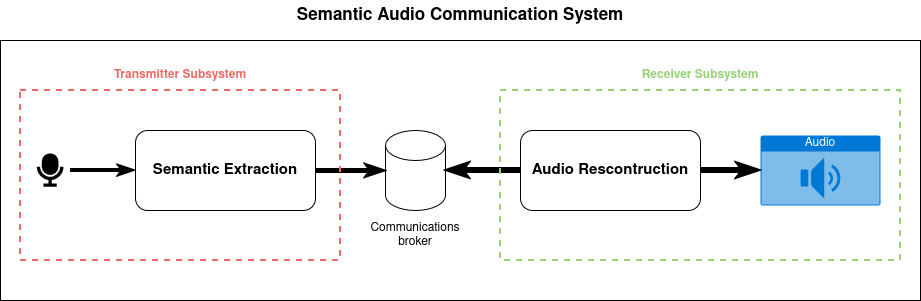
\includegraphics[width=\textwidth]{midterm-pres-images/sys_concept.png}
\end{figure}
\end{frame}


\section{System Breakdown Structure}
\begin{frame}{System Breakdown Structure}
\transdissolve
\small
\begin{figure}[H]
	\centering
	\includesvg[width=\textwidth]{midterm-pres-images/SBS.drawio.svg}
\end{figure}
\end{frame}

\section{Functional Architecture}
\begin{frame}{Functional Architecture}
\transdissolve
\small
\vspace{-10pt}	
\begin{figure}[H]
	\centering
	
\includegraphics[width=\textwidth]{midterm-pres-images/func-arch.png}
\end{figure}
\vfill
\end{frame}

\section{Work Breakdown Structure + Gantt}
\begin{frame}{Work Breakdown Structure + Gantt}
\transdissolve
\small
\begin{figure}[H]
	\centering
	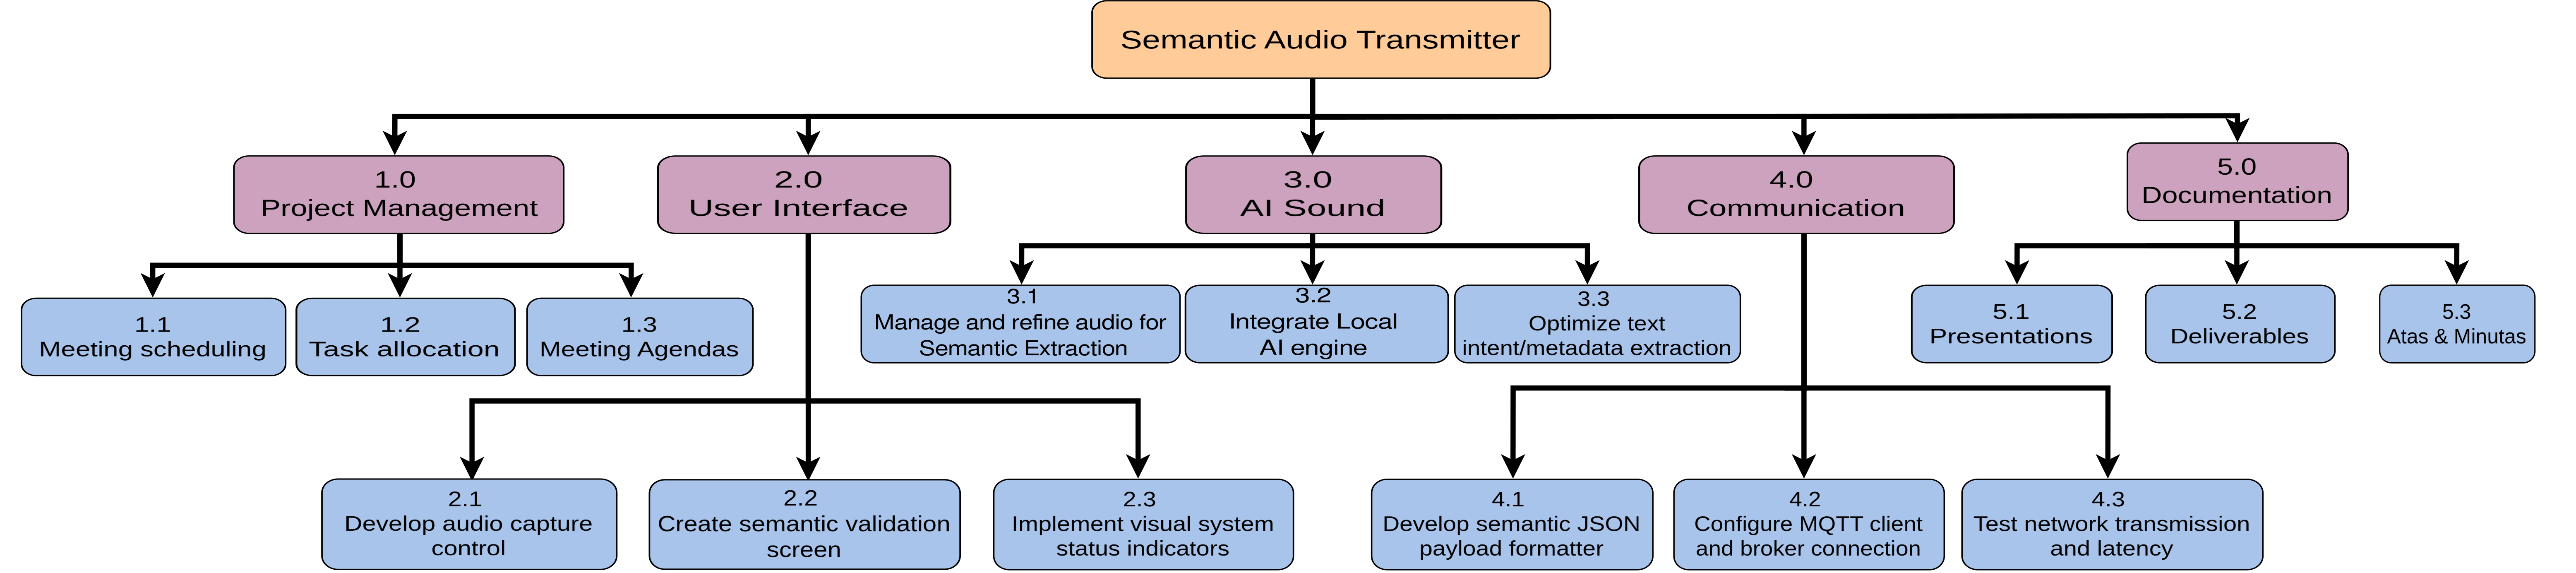
\includegraphics[width=\textwidth , height=7cm]{midterm-pres-images/WBS.drawio.png}
\end{figure}
\end{frame}

\begin{frame}{Gantt Chart}
	\transdissolve	
	\begin{figure}[H]
		\centering
		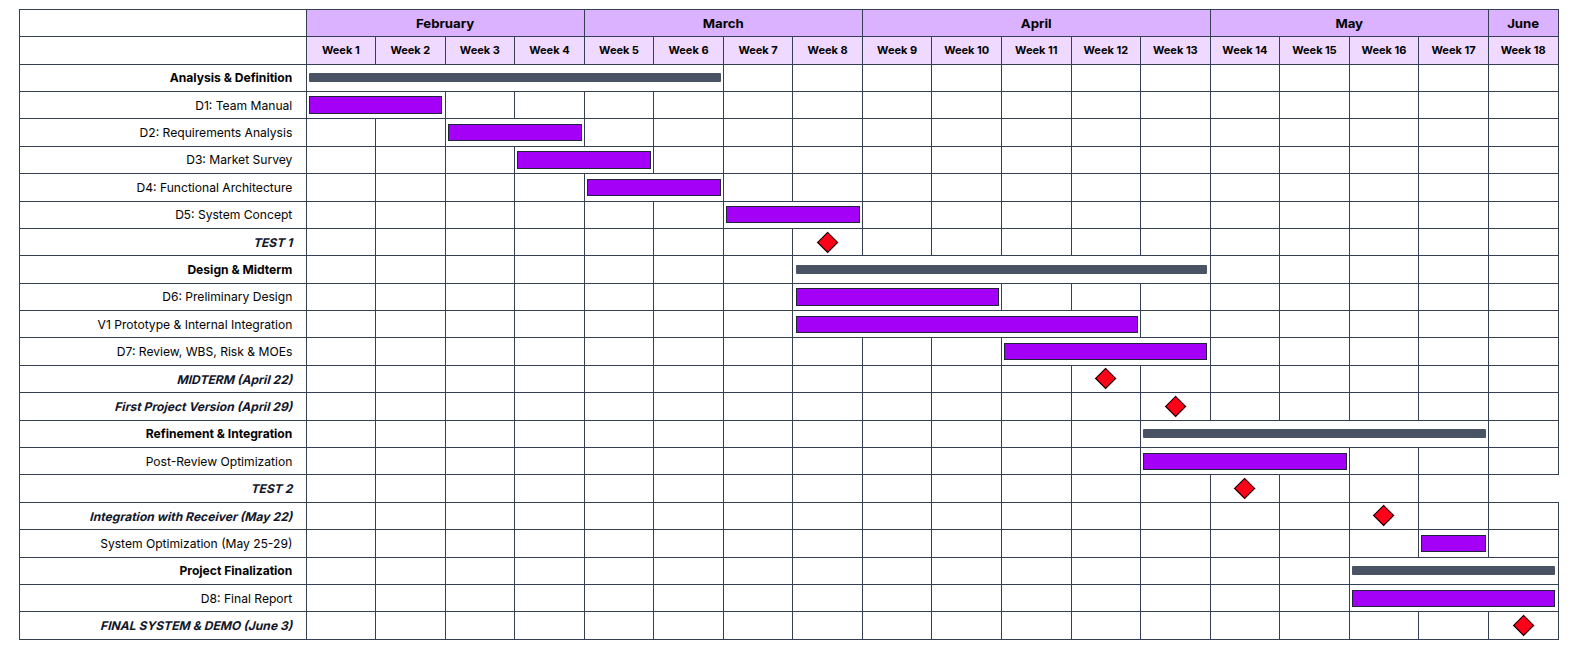
\includegraphics[width=\textwidth]{midterm-pres-images/Gantt.png}
	\end{figure}
\end{frame}

\section{Measures of Effectiveness and Performance}
\begin{frame}{Measures of Effectiveness and Performance}
\transdissolve
\small
\vspace{-15pt}
\begin{figure}[H]
	\centering
	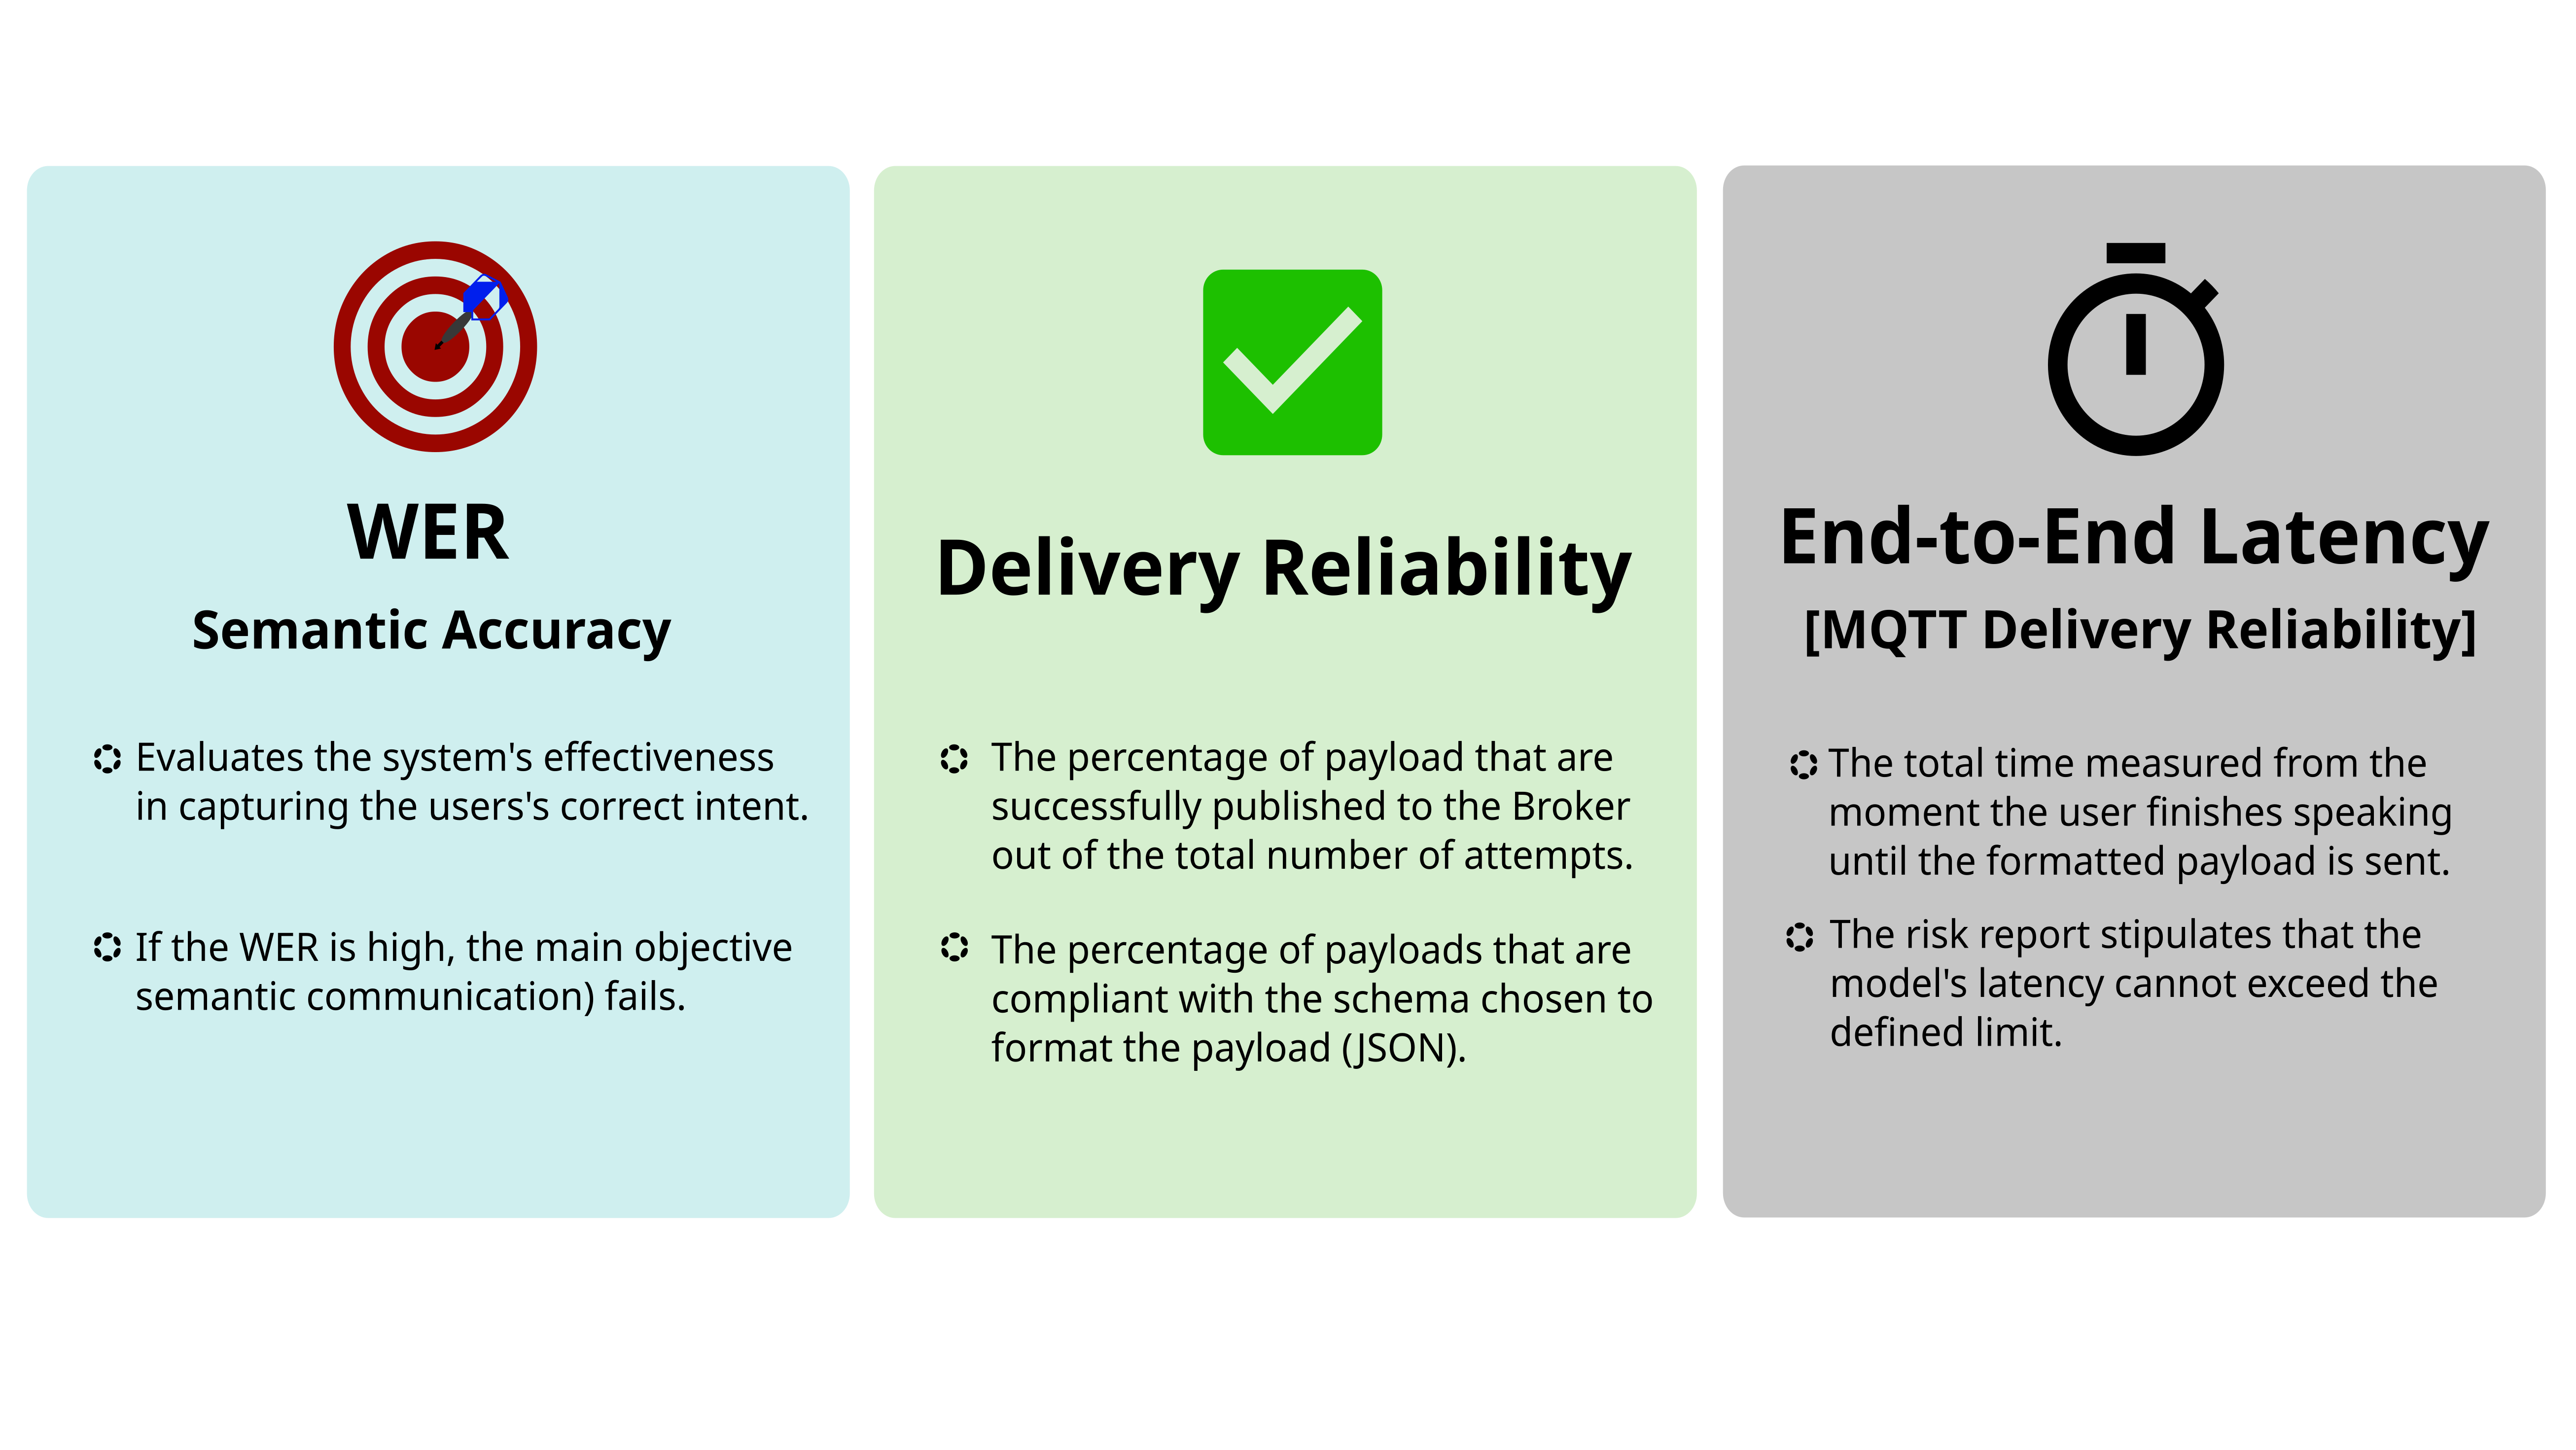
\includegraphics[width=\textwidth]{midterm-pres-images/moe-mop.png}
\end{figure}
\end{frame}

\section{Risk Management}
\begin{frame}{Risk Management}
\transdissolve
\small
\begin{minipage}{0.8\textwidth}
\vspace{-20pt}
\begin{figure}[H]
	\centering
	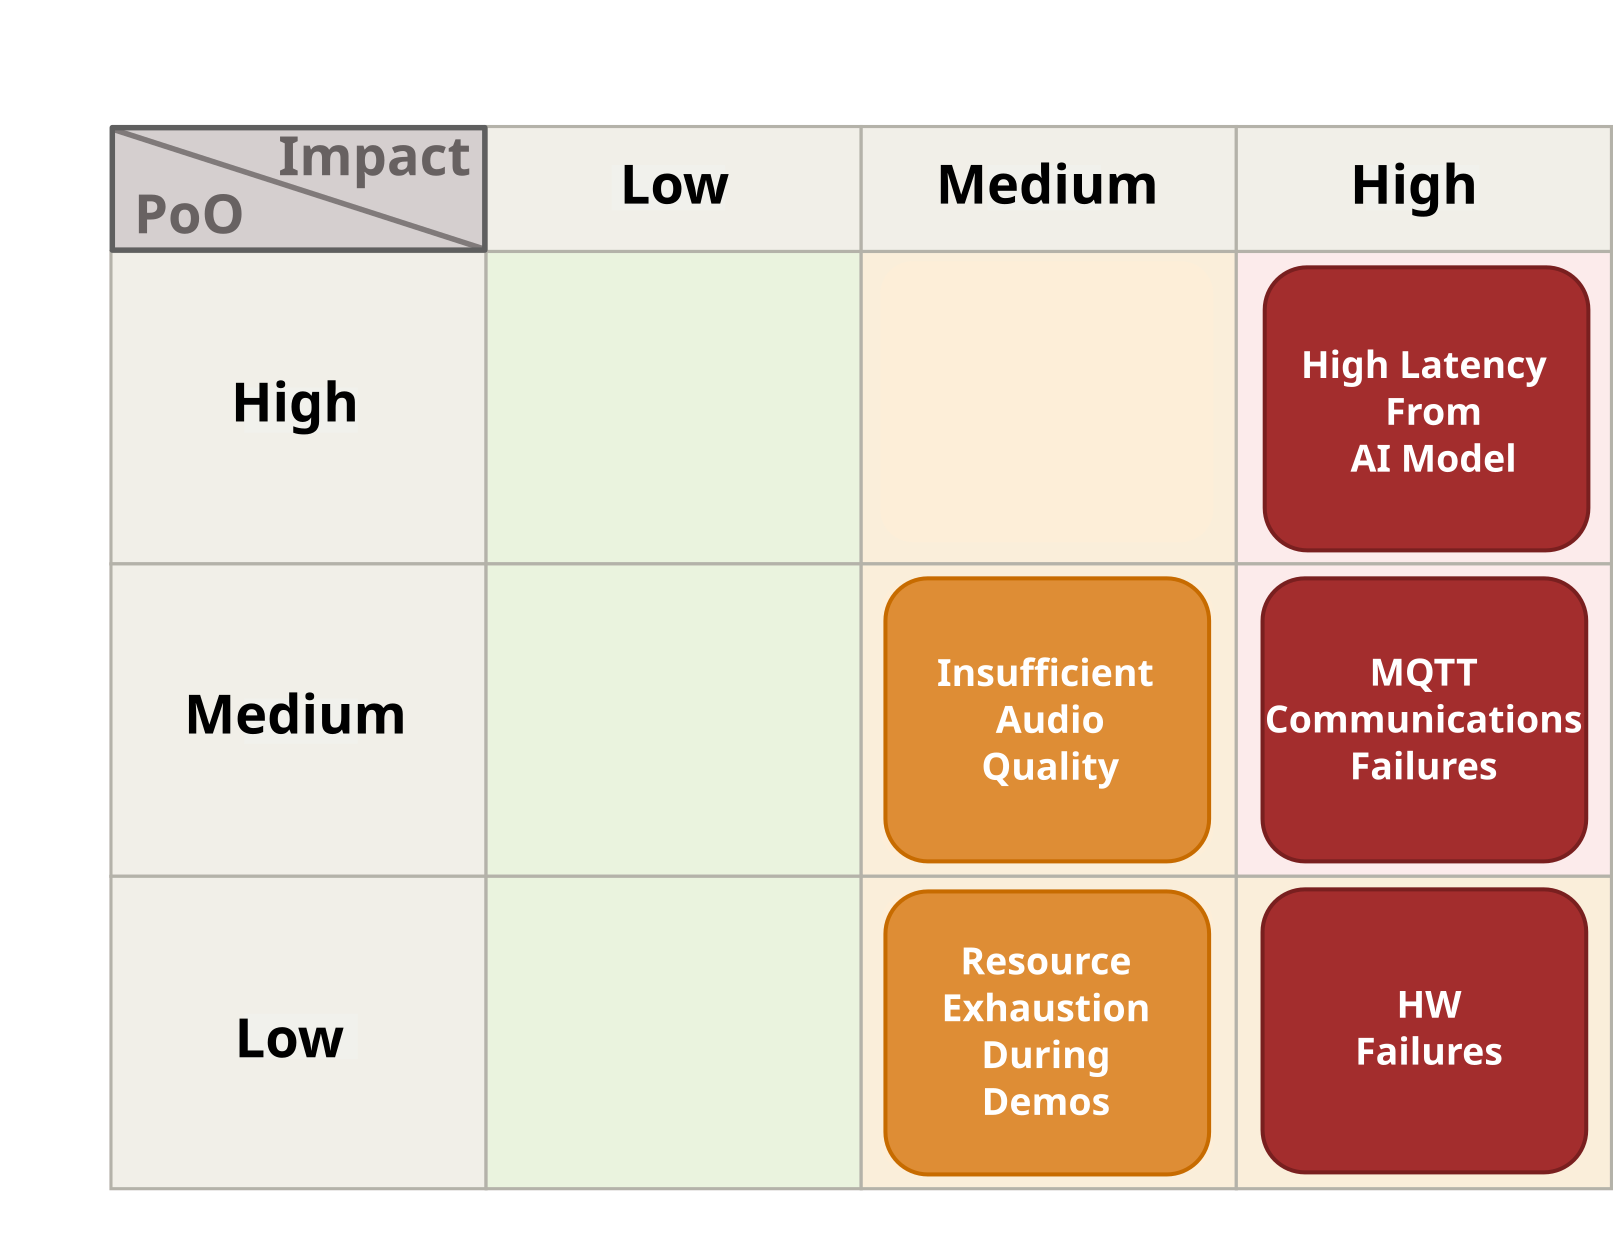
\includegraphics[width=\textwidth, height=8.2cm]{midterm-pres-images/risk-table.png}
\end{figure}
\end{minipage}
\begin{minipage}{0.19\textwidth}
\vspace{16pt}
\hspace{3pt}\textbf{PoO} - Probability of Occurence
\end{minipage}
\end{frame}

\section{Conclusion}
\subsection{Internal Evaluation}
\begin{frame}{Internal Evaluation}
\transdissolve
\small
\begin{figure}
	\centering
	\includesvg[width=0.85\textwidth]{midterm-pres-images/internal-eval.svg}
\end{figure}
\end{frame}

\subsection{Next Steps}
\begin{frame}{End of Semester Plan}
\transdissolve
\small
\begin{figure}[H]
	\centering
	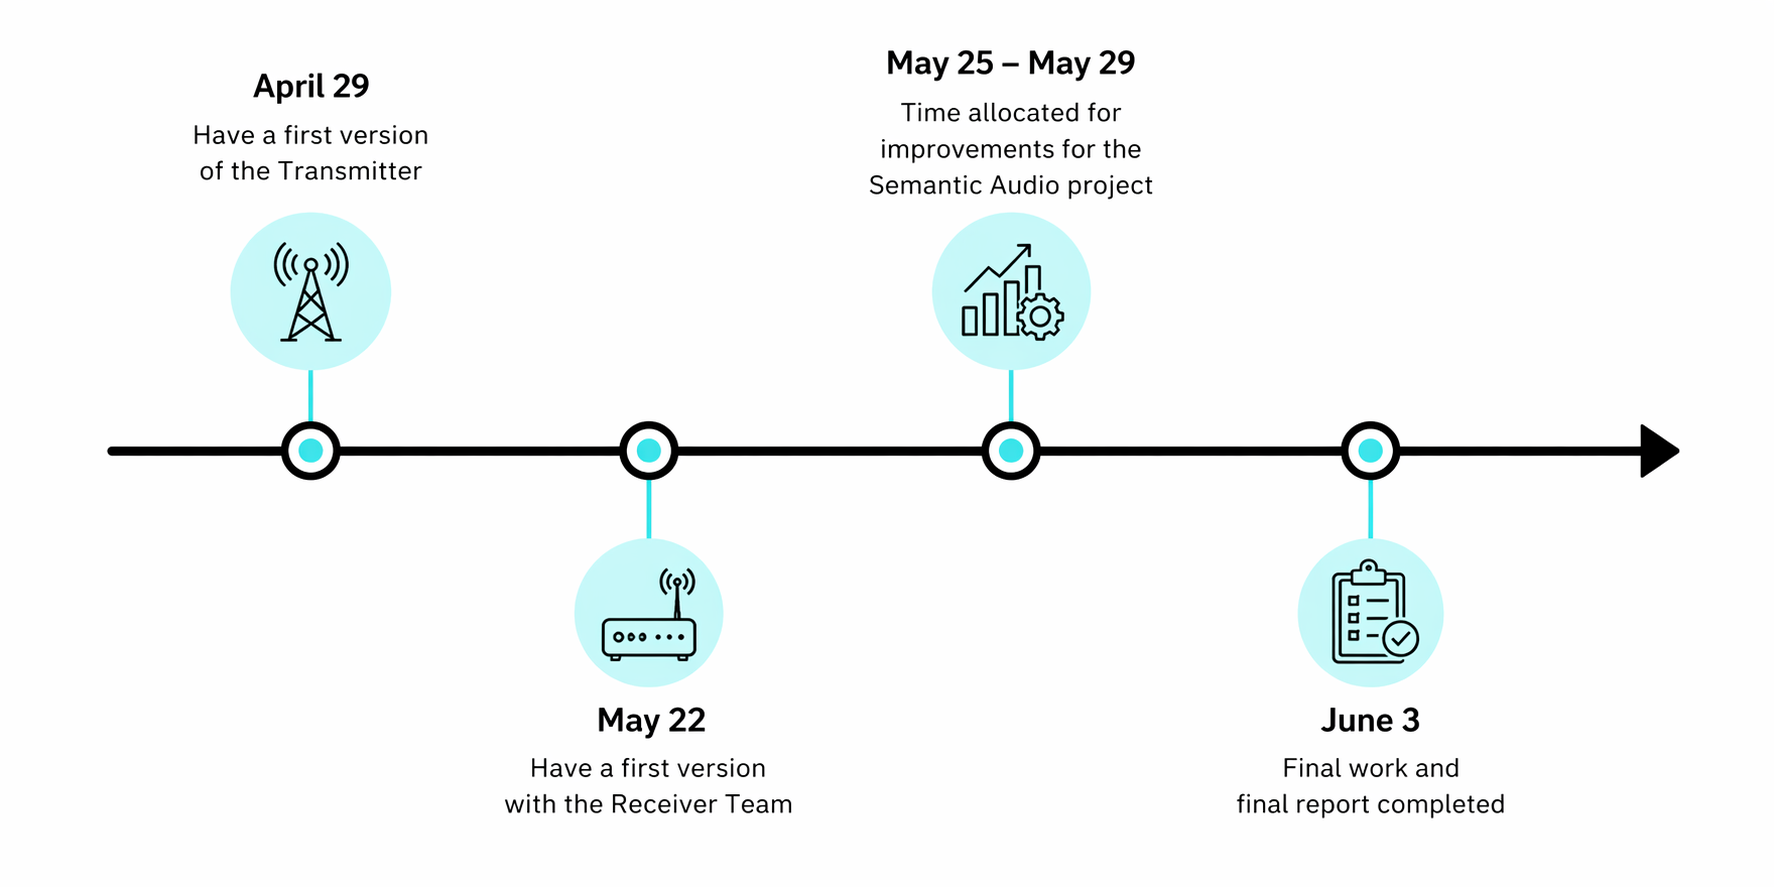
\includegraphics[width=\textwidth]{midterm-pres-images/timeline.png}
\end{figure}
\end{frame}

\begin{frame}
	\transdissolve
	\begin{center}
		\huge Thank You for Your Attention!
	\end{center}
\end{frame}

\begin{frame}[allowframebreaks]{References}
\footnotesize
\nocite{*}
\bibliographystyle{plain}
\bibliography{references}
\end{frame}

\end{document}
